 %% Le rapport final reprendra le rapport de conception (corrigé)
  % + mise en œuvre (réalisations) + manuels instal/utilisateur
  % + jeu de tests
  % + pblms rencontrés, etc.)

%%configuration de listings
\lstset{language=C} % TODO - configurer correctement la coloration de code

\section{Implémentation et mise en œuvre}
 
  \subsection{Choix de la technologie}
    \paragraph{}
     Pour la réalisation de notre projet, le choix nous a été donné entre 
     socket et RPC pour la communication entre machines. 
     Nous avons porté notre choix sur RPC grâce à différents  avantages 
     qu'il présente par rapport et à certains critères que nous avons définis. 

     \paragraph{}
     \noindent Facilité de programmation :
     RPC (appel de procédures à distance) cache la complexité des protocoles 
     de communication et permet la génération automatique de code (à l'aide
     de RPCGEN) pour le client et pour le serveur qui couvre la communication 
     (les talons ou souches). Les appels sont fait comme des appels de procédures
     en local (sauf qu'il ne permet pas le passage par adresse).
     
     \paragraph{}
     \noindent Portabilité et Héterogenéité :
     RPC utilise le standard XDR pour l'envoie de messages entre machines
     
 \subsection{Génération du code RPC}
    \paragraph{utilisation de rpcgen}
    Nous avons dans un premier temps procédé à la génération du code rpc
    en utilisant l'outil rpcgen. Dans le fichier \verb"PlacementReparti.x" nous
    avons défini les structures de données de notre programme (tel que
    vu dans la Figure 11). A cela nous avons spécifié dans l'interface
    les procédures qui seront appelés à distances  tel que présenté
    ci-dessous.
    
    
    \paragraph{}
    \noindent Procédures distantes pour une machine esclave :
    
    \begin{verbatim}
      unsigned long quiEstPlusGrand(unsigned long) = 1;
      unsigned long tuConnaisMaitre() = 2;
      string collecterDonneesMachine() = 3;
      void jeSuisInitialise() = 4;
      int recolterCharge() = 5;
      bool_t executerDistante(ProgrammeExporte) = 6;
      void terminerProgramme(RetourFinExecution) = 7;
    \end{verbatim}
    
    \paragraph{}
    \noindent Procédures distantes supplémentaire pour une machine maître :
    \begin{verbatim}
      string collecterDonneesMachines() = 1;
      bool_t enregistrerEsclave(MachineEsclave) = 2;
      unsigned long choisirMachineDistante() = 3;
    \end{verbatim}
    
    \paragraph{Organisation des fichiers}
    A partir des fichier générées par rpcgen nous avons réorganisé le code
    afin de le placer dans des fichier correspondant aux interfaces défini
    précédemment. Ainsi nous avons un fichier header par module (information,
    transfert, localisation et IHM), ainsi qu'un dernier fichier pour 
    gérer le démarrage de notre application (\verb"InitialiserPlacement.h").
    
    Nos fichiers sources sont organisés en trois parties. Une partie 
    contenant les procédures d'appel côté client (tel que généré par
    rpcgen), situé dans des fichiers nommés \verb"ModuleXXXAppel.c". Les deux
    autres parties sont situés dans les fichiers sources (\verb"ModuleXXX.c").
    Chaque ficher de module contient d'une part les procédures locales à
    une machine et d'autre part les procedures distantes (côté serveur).
    
    % TODO bonus - mettre un schéma d'arborescence
  
    
  \subsection{Integration d'une machine au placement}
    \paragraph{}
    Nous avons choisi dans un premier temps de nous intéresser à
    l'intégration d'une machine dans notre système afin de pouvoir
    travailler sur un base minimale de notre application et d'étendre au
    fur et à mesure les fonctionnalités. Le choix à été fait de rendre
    totalement transparent l'intégration d'une machine au système, pour
    cela nous avons utilisé la fonction broadcast de RPC. la procédure 
    \verb"InitialiserPlacementReparti" s'occupe de determiner par un premier
    broadcast si il existe déjà un maître actif sur le réseau. S'il n'y
    a pas de réponse, la procédure lance une élection afin d'élire un
    nouveau maître.
    Une fois le type de n\oe{}ud déterminé, la procédure ce charge
    d'enregistrer les fonctions qui pourront être appelées à distance.
    Il ne reste plus alors qu'à lancer le serveur RPC avec la fonction RPC
    \verb"svc_register" et d'attendre les requêtes des autres machines du placement 
    avec la fonction RPC \verb"svc_run". 
  
  \subsection{Interface (IHM)}
    \paragraph{}
    L'interface utilisateur que nous avons créée s'inspire très
    fortement de la commande \verb"ftp". Notre binaire se lance sans argument,
    une fois l'étape d'integration passée, notre programme laisse la 
    main à l'utilisateur où il pourra tapez une des 5 commandes de notre
    application (EXECUTE, QUIT, KILL, ADMIN ou HELP). Pour parser la
    commande nous avons utilisé les fonction de la librairie standard C
    \verb"fgets", \verb"strtok" et \verb"strcmp". 
    Étant donné que nous avons lancé le serveur RPC avant d'attendre les
    commandes de l'utilisateur, nous avons dû créer un nouveau thread.
    Ainsi la fonction \verb"entrerCommande", qui se charge de parser les 
    commandes et d'aiguiller vers les fonctions adéquats, est lancé dans
    un thread séparé.
  
  \subsection{Exécution d'un programme}
    \paragraph{}
    L'execution d'un programme (ou tâche) se fait par un appel des 
    fonctions \verb"fork" puis \verb"exec", en passant en parametre la ligne de
    commande donné par l'utilisateur. Chaque machine possède deux liste
    de tâche : une liste des tâches propres à la machines, qu'elles 
    soient éxecutées localment ou exportés sur une machine distante ; et
    une liste des tâches importées. On aura, associé à ces deux listes, 
    deux compteur pour le nombre d'entrées qui faciliteront la gestion.
    
    \subsubsection{Exécution locale}
    
      \paragraph{}    
      Un des principal problème à résoudre a été la détection de la
      terminaison d'un programme. Étant donné que la fonction \verb"wait" est
      bloquante nous ne pouvons pas l'executer dans le même thread que
      notre programme principal. Nous avons donc décidé de créer un
      thread pour chaque tâche éxecuté localement qui se chargera de 
      traiter la fin du processus fils. 
      
      Une autre solution envisagé était de redéfinir le signal
      SIGCHLD mais celle-ci n'était pas satisfaisante car il est
      impossible d'attendre le processus de pid voulu.

      
      % TODO mettre l'image sur github 
      \begin{figure}[h!]
        \centering
        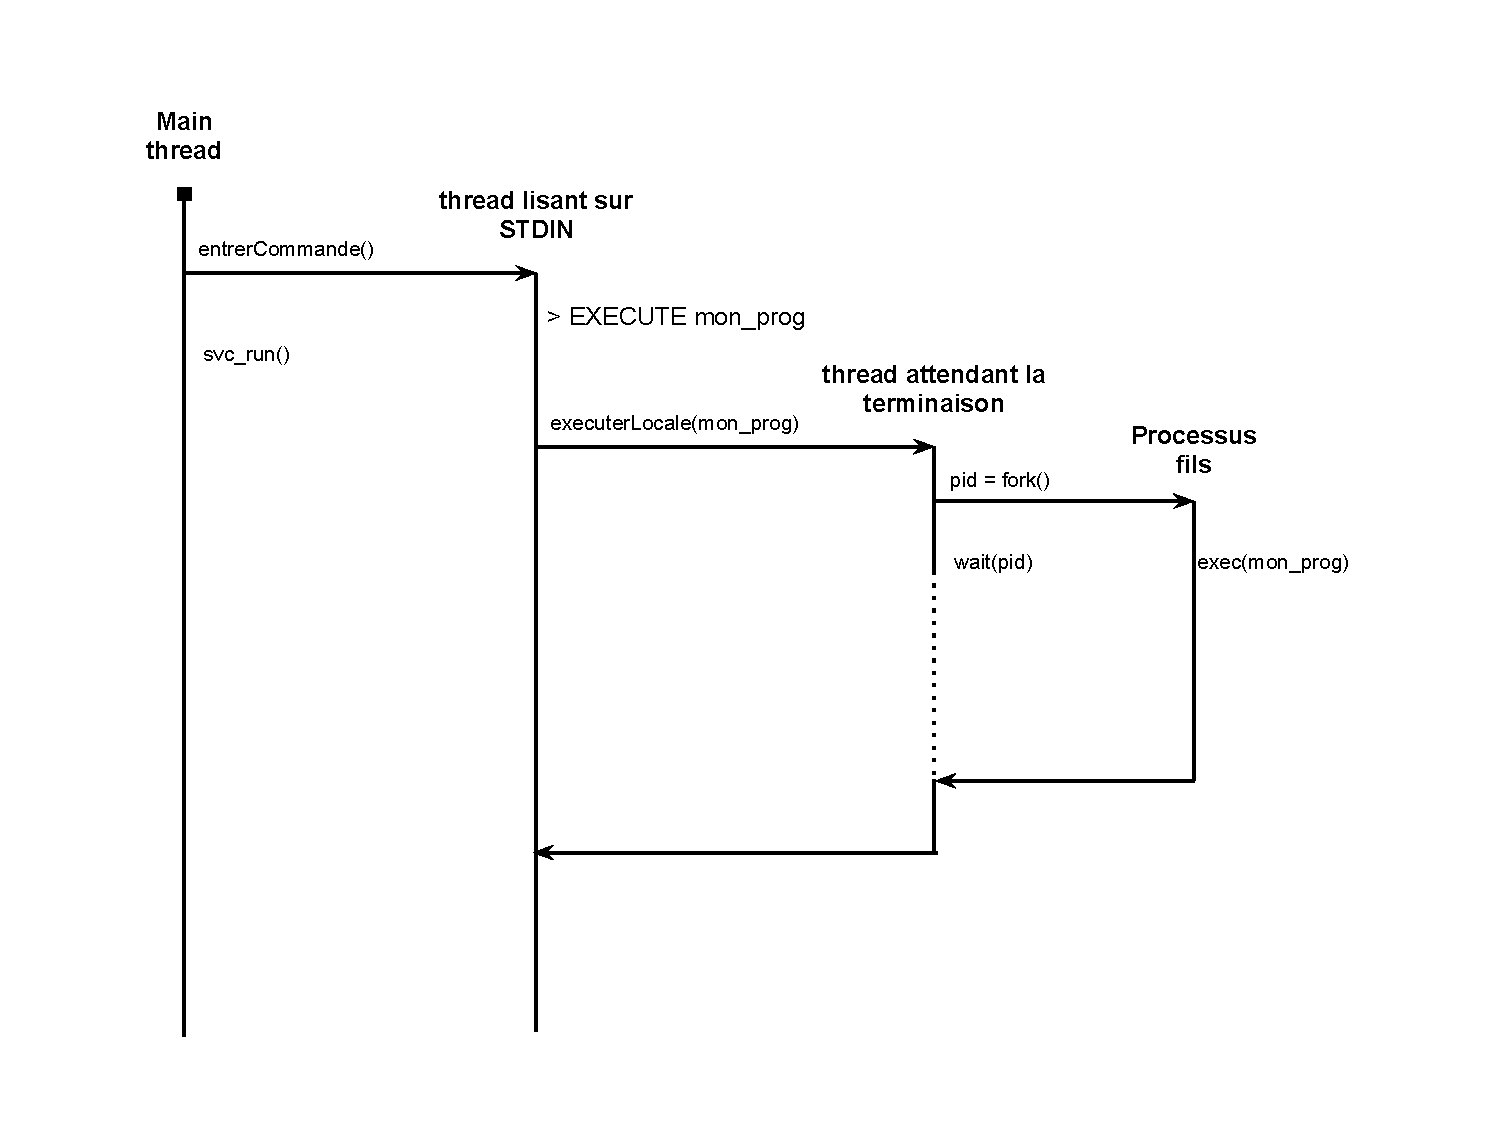
\includegraphics[scale=0.6]{img/execution_locale.pdf}
        \caption{Threads et processus impliqués dans l'éxecution d'un 
                 programme sur une machine locale}
      \end{figure}
    
  \subsubsection{Exécution à distance}
    \paragraph{}
    L'exécution à distance se fait par appel de la fonction 
    \verb"executerDistance" qui se charge de transmettre les informations
    nécessaire à l'éxecution du programme. De la même manière que lors
    de l'exécution locale, la machine (distante) exécutant le programme 
    créera un thread d'attente qui se chargera de notifier la machine 
    appelante. Du fait de ce choix, la notification de terminaison est 
    asyncrone : la machine choisie pour l'éxecution se chargera de 
    notifier la fin du programme par l'appel de la procédure distante 
    \verb"terminerProgramme".
    
    
    
    
    
    % TODO - Redirection E/S : pas implementé
    % L'execution étant à distance, les entrées/sorties sont rédirigés 
    % afin que les affichages se fassent sur la machine appelante.
    
    \newpage
    
    % TODO mettre l'image sur github
    \begin{figure}[h!]
      \centering
      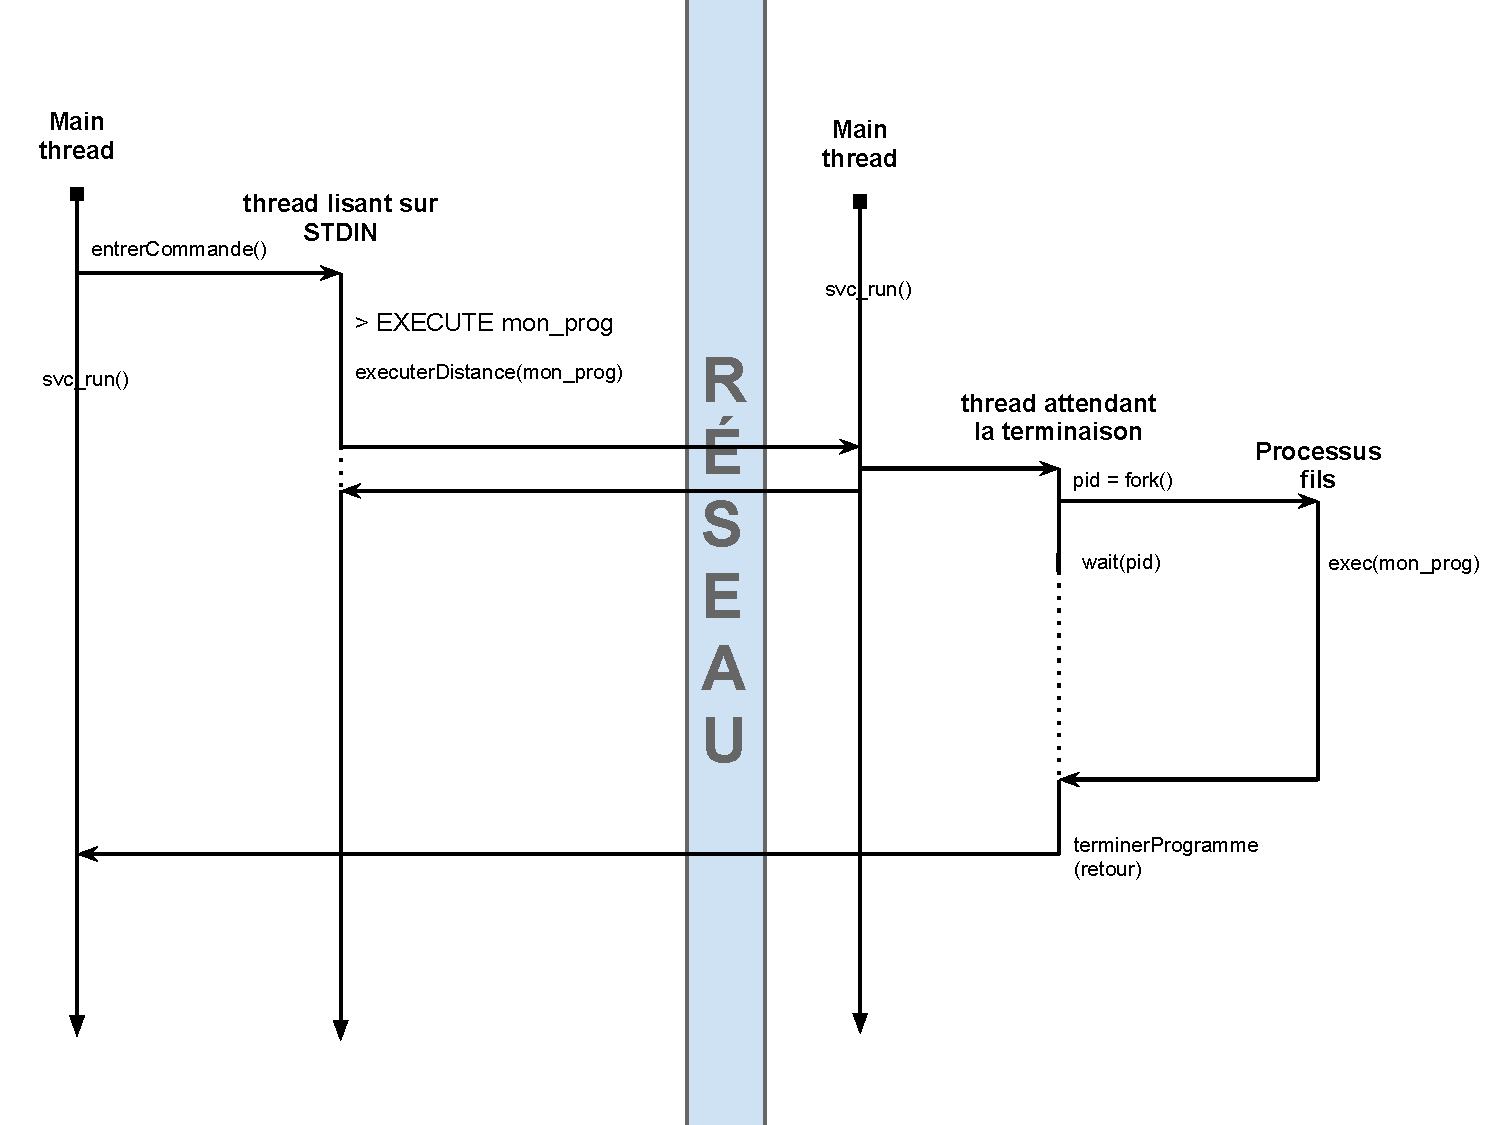
\includegraphics[scale=0.6]{img/execution_distante.pdf}
      \caption{Threads et processus impliqués dans l'éxecution d'un 
               programme sur une machine distante}
    \end{figure}

  \subsection{Calcul de la charge}
    \paragraph{}
    Étant donné que nous n'avons pas d'accès sur les informations des 
    processus au niveau noyau, nous avons utilisé les informations 
    disponibes en lecture dans le dossier \verb"/proc". A partir de ces 
    informations, nous avons établit la définition suivante :
    la charge correspont au nombre de processus utilisateur existant sur 
    la machine. Nous n'avons pas pris en compte la puissance du 
    processeur, notre environnement de test (salle de l'ARI) étant 
    constitué de machines de même puissance. La fonction de calcul pourra 
    tout de même être redefine afin de prendre en compte cette 
    problématique.
  
  \subsection{Choix de la machine}
    \paragraph{} 
    Nous avons implémenté 2 modes de  répartition : partage ou 
    équilibrage. Le choix du mode est fait "en dur" au moment de la 
    compilation mais il a été pris en compte la possibilité d'évolution 
    vers un choix au lancement du système, voir un changement pendant 
    l'execution du programme.
    
    \paragraph{Partage} 
    Dans le cas Partage, la décision se fait en partie localment. Si la 
    charge est inférieure au seuil, l'éxecution est locale, sinon on 
    demande au maître l'identité d'une machine pouvant exécuter la tâche
    à répartir. Le maître récoltera alors les charges des esclaves à 
    l'aide d'un broadcast de la procédure RPC \verb"recolterCharge", 
    puis choisira la première machine qui possède une charge inférieure 
    au seuil.
    
    \paragraph{Équilibrage}
    Dans le cas équilibrage, on interogerra systématiquement le maître 
    pour obtenir l'identité de la machine la plus apte.
    Lorsque le maître est interrogé il effectue un récolte de toutes les 
    charges de la même manière que pour le partage. Une fois la table 
    des charges à jour, le maître prend ça décision. Il choisira 
    systématiquement la machine la moins chargé.
    
  \subsection{Consultation de l'état de machines}
    % La consultation se fait par la commande ADMIN.
    Nous avons implémenté deux possibilité consultation : consultation 
    de l'état de toutes les machines (globale) et consultation de l'état
    d'une seule machine (locale).
    
    \paragraph{Consultation locale}
    La consultation locale correspont à un appel de la procédure distante 
    \verb"collecterDonneesMachine" sur la machine spécifié par 
    l'utilisateur (à l'aide de la commande ADMIN). Cette procédure se 
    charge de créer une chaine de caratères formaté pour l'affichage à
    partir des données locales (état, programmes exportés et programmes
    importés). La machine appelante se contente alors d'afficher la 
    chaine obtenue.
    % TODO
    % Voici un exemple d'affichage obtenu :
     
    
    \paragraph{Consultation globale}
    La consultation globale se fait par l'appel d'une procédure à 
    distance sur le maître pour obtenir l'état de l'ensemble des 
    machines du placement. Le maître effectue alors un collecte locale 
    sur l'ensemble des machines du système, puis agrège les chaînes 
    obtenu afin d'obtenir un texte prêt à être affiché.
    
    % TODO - pas codé
    %\paragraph{}
    %Afin de pouvoir observer le comportement du sysème, nous avons dans 
    %un seconde temps rendu l'affichage dynamique avec un fréquance de 
    %rafraichissement de 1 seconce. Pour cela nous avons utilisé la 
    %fonction alarm et redefini le signal SIGALRM (à l'aide de 
    %\verb"sigaction") sont utilisés pour raffraîchir l'affichage en
    %faisant une réexecution de la procedure à interval de temps régulier.
    
    
    \subsection{Retrait d'une machine}
    Comme vu précédemment, nous avons implémenté deux façon de quitter 
    le système. 
    
    \paragraph{}
    La première (commande \verb"KILL") n'attend pas la terminaison des 
    tâche mais notifie tout de même le maître de l'arrêt de la machine.
    Lors d'un arrêt ce ce type, la machine signal au maître sa 
    terminaison puis termine toutes les tâches en cours sur elle-même.
    Le maître notifira toutes les autres machines du placement afin 
    qu'elles gèrent elles-même la terminaison des tâches de la machine 
    venant de quitter.
    
    \paragraph{}
    La seconde (commande \verb"QUIT") attends la terminaison de toutes 
    les tâches, celles en cours sur la machine même mais aussi celles qu'elle 
    aura exporté sur d'autres machines. Pour cela la machine signalera 
    dans un premier temps au maître qu'elle n'accepte plus de tâche. 
    A chaque terminaison de tâche on testera nos compteurs afin de 
    savoir si le programme peut s'arrêter.
    
    % TODO
    \subsection{Gestions des pannes}
    
\section{Test}   
  \subsection{Environnement de test}
  
\section{Manuel d'utilisation}
   \subsection{Paramétrage et Compilation}
    \paragraph{}
    Le dossier de l'application présente les sous dossiers de notre code
    source : src (les xxx.c), include (les xxx.h) et bin (le fichier
    PlacementReparti). Dans le répertoire il y a un fichier Makefile qui
    permet la compilation et un fichier README.txt qui constitue notre
    manuel d'utilisation.

    \paragraph{}
    Par défaut, le type de répartition considéré est partage de charge,
    donc si on voudrait utiliser plutôt l'équilibrage de charge, il faut
    modifier les sources. Pour celà, il faut modifier dans le code
    source du fichier ModuleTransfert.c, situé dans le sous dossier src,
    la ligne typeRepartion = PARTAGE par typeRepartiton = EQUILIBRAGE.

    \paragraph{}
    Pour créer un éxecutable du programme, il faut ouvrir un terminal et 
    de se déplacer dans le dossier de l'application et, ensuite, 
    d'entrer la commande "make -f Makefile". L'exécutable est créé et se 
    situe dans le sous dossier bin.
    
    \subsection{Démarrage du placement}
    \paragraph{}
     Pour démarrer le placement, il faut se deplacer dans le sous 
     dossier bin du dossier du programme et d'entrer la commande
     "./PlacementReparti". Un message d'attente d'intégration ou une 
     invite d'entrée de commande ">" s'affiche. Dans le cas du message 
     d'attente, il faut patienter que l'invite soit affiché.
     
     \paragraph{}
     A l'aide de la commande HELP, on a la possibilité de connaitre tous 
     les commandes du placement  que voici : EXECUTE, QUIT, KILL, 
     ADMIN ou HELP. 
     \begin{verbatim}
       > HELP
     \end{verbatim}
     
     
    \subsection{Exécution d'un programme}
      \paragraph{}
      On exécute un programme avec la commande EXECUTE en lui fournissant 
      en paramètre le nom du programme et ses paramètre :
      \begin{verbatim}
        > EXECUTE /programme param1 param2 ...
      \end{verbatim}
      
      \paragraph{}
      La fin de l'exécution du programme est signalée.
      
       
      \subsection{Retrait d'une machine}
      \paragraph{}
      La commande QUIT entrée, la machine attend terminaison des 
      programmes exécutés sur elle des autres machines et, à la fin, elle 
      signale le retrait de la machine du placement.
      \begin{verbatim}
        > QUIT
      \end{verbatim}     
      
      \paragraph{}
      La commande KILL quant à elle met fin immédiatement les programmes 
      et retire la machine du placement
      \begin{verbatim}
        > KILL
      \end{verbatim}
      
      
    \subsection{Consulter l'état des machines}
      \paragraph{}
      La commande ADMIN nous permet de consulter l'état d'une machine ou 
      de l'ensemble de machines du placement. 
      
      \paragraph{}
      D'une machine, il faut entrer la commande avec un paramètre 
      l'adresse de la machine :
      \begin{verbatim}
        > ADMIN 192.168.1.4
      \end{verbatim}      
      
      \paragraph{}
      De toutes les machines, il faut entrer la commande avec le 
      paramètre étoile ou sans :
      \begin{verbatim}
        > ADMIN *
        
        > ADMIN
      \end{verbatim}
      
